
\chapter{Finite Difference Schemes for the Heat Equation}\label{chap7}

\section{Introduction}\label{chap7:sec7.1}

In this\pageoriginale, we view various examples of finite difference
schemes for the heat equation, $u_t - u_{xx} = 0$. We study the
stability and consistency of these schemes. We sketch the proof of
convergence, using stability and consistency. Finally we sketch
briefly how to deal with variable coefficients and with non-linearity.

\section{Four Schemes for the Heat Equation}\label{chap7:sec7.2}

Let us assume henceforth a uniform mesh of steps $\Delta x$ and
$\Delta t$. We use the notation
\begin{equation*}
u^n_i = u(i \Delta x, \;n \Delta t).
\tag{7.1}\label{eq7.1}
\end{equation*}
We now proceed to give four different schemes for the heat equation.

\begin{exam}\label{chap7:exam7.1}
{\em An explicit scheme}.

The scheme reads as
\begin{equation*}
\frac{u^{n+1}_i - u^n_i}{\Delta t} - \frac{1}{\Delta x^2} (u^n_{i+1} -
2 u^n_i + u^n_{i-1})  = 0.\tag{7.2}\label{eq7.2}
\end{equation*}
This scheme is clearly explicit. Applying the Fourier transform as in
Sec. \ref{chap6:sec6.3}, we get
\begin{align*}
b(\xi) & = \frac{1}{\Delta t}\\
c(\xi) & = \frac{1}{\Delta t} - \frac{2}{\Delta x^2} + \frac{1}{\Delta
x^2} (e^{i\xi \Delta x} + e^{-i \xi \Delta x})
\end{align*}
which gives the cofficient of amplification
\begin{equation*}
a(\xi) = \frac{c(\xi)}{b(\xi)} =1 - \frac{4\Delta t}{\Delta x^2}
\sin^2 (\frac{\xi \Delta x}{2}). \tag{7.3}\label{eq7.3}
\end{equation*}\pageoriginale
Hence 
\begin{equation*}
\hat{u}^{n+1} (\xi,t) = a(\xi) \hat{u}^n (\xi,t)\tag{7.4}\label{eq7.4}
\end{equation*}
with $a(\xi)$ as in (\ref{eq7.3}).

Using the stability criteria of Sec. \ref{chap6:sec6.3}, viz. $|a(\xi)| \leq 1$ for
all $\xi$, we see that this scheme is stable if and only if 
\begin{equation*}
\frac{2\Delta t}{\Delta x^2} \leq 1.
\tag{7.5}\label{eq7.5}
\end{equation*}

Expanding the left-hand side of (\ref{eq7.2}), for the exact solution $u$ of
the heat equation, by means of a Taylor expansion about $(i \Delta
x. n \Delta t)$, we get
$$
\frac{\partial u}{\partial t} + \frac{\Delta t}{2}  \frac{\partial^2
  u}{\partial t^2} + \ldots - \left[ \frac{\partial^2 u}{\partial x^2}
  + \frac{\Delta x^2}{ 12} \frac{\partial^4 u}{\partial x^4} + \ldots
  \right] 
$$
and since $u$ satisfies the heat equation, we see that, for the
explicit scheme, the {\em error of discretization} is the order
$O(\Delta t+ \Delta x^2)$.

Note that by (\ref{eq7.5}), in order to get a stable scheme, one needs $\Delta
t$ to be of the order of $\Delta x^2$ and then the overall error of
discretization is of order $O(\Delta t)$. However, when we combine the
heat equation with other equations, one needs $\Delta t$ to be of the
order of $\Delta x$. Thus one feels the need for other schemes. As
already remarked in Sec. \ref{chap6:sec6.3}, explicit schemes are not generally
unconditionally stable while implicit schemes are. Thus one generally
uses an implicit scheme.
\end{exam}

\begin{exam}\label{chap7:exam7.2}
{\em An implicit scheme}

This scheme reads as
\begin{equation*}
\frac{u^{n+1}_i - u^n_i}{\Delta t} - \frac{1}{\Delta x^2}
\left[u^{n+1}_{i+1} - 2u^{n+1}_i + u^{n+1}_{i-1} \right] = 0
\tag{7.6}\label{eq7.6}
\end{equation*}
Again\pageoriginale one has the relation (\ref{eq7.4}) with $a(\xi)$ defined
by 
\begin{equation*}
a(\xi) = \left[ 1+ \frac{4\Delta t}{\Delta x^2} \sin^2 \left(\frac{\xi
    \Delta x}{2}\right) \right]^{-1}\tag{7.7}\label{eq7.7}
\end{equation*}
and as this always has absolute value $\leq 1$, the scheme is {\em
  unconditionally stable}, i.e. there is no relation between $\Delta
x$ and $\Delta t$ for stability. Once again, using a Taylor expansion,
one finds the error of discretization to be of order $O(\Delta x^2 +
\Delta t)$.
\end{exam}

Though this scheme is unconditionally stable, one would prefer an
error of discretization of order $O(\Delta x^2 + \Delta t^2)$. To this
end, we present two such schemes 

\begin{exam}\label{chap7:exam7.3}
{\em Richardson's Scheme.}
This is, in truth, a 3-level scheme given by
\begin{equation*}
\frac{u^{n+1}_i - u^{n-1}_i}{\Delta t} - \frac{1}{\Delta x^2} \left[
  u^n_{i+1} - 2 u^n_i + u^n_{i-1}   \right] = 0. \tag{7.8}\label{eq7.8}
\end{equation*}

One reduces this to a {\em system} of two equations by the
substitution $v^n_i = u^{n-1}_i$ for all $i$. By applying the Fourier
transform, one finds that the spectral radius of the matrix
$B^{-1}C(\xi)$ is always larger than 1, (Exercise !) and hence the
scheme is {\em always unstable}.
\end{exam}

\begin{exam}\label{chap7:exam7.4}
The Crank-Nicolson Scheme. The scheme is given by
\begin{equation*}
\frac{u^{n+1}_i - u^n_i}{\Delta t} - \nabla^2 \left(\frac{u^{n+1} +
  u^n}{2}\right) = 0 \tag{7.9}\label{eq7.9}
\end{equation*}
where
\begin{equation*}
\nabla^2 v = \frac{1}{\Delta x^2} (v_{i+1} - 2v_i + v_{i-1}). 
\tag{7.10}\label{eq7.10}
\end{equation*}
Once again one has the relation (\ref{eq7.4}) with 
\begin{equation*}
a(\xi) = \frac{1-\dfrac{2\Delta t}{\Delta x^2} \sin^2 \left(\dfrac{\xi
    \Delta x}{2} \right)}{1 + \dfrac{2\Delta t}{\Delta x^2} \sin^2
  \left(\dfrac{\xi \Delta x}{2}\right)} \tag{7.11}\label{eq7.11}
\end{equation*}
and this scheme is seen to be unconditionally stable. The order of the
error of discretization\pageoriginale is easily checked to be
$O(\Delta x^2 + \Delta t^2)$. 
\end{exam}

\section{Consistency}\label{chap7:sec7.3}

The consideration of the order of the error of discretization leads to
the following definitions.

\begin{Definition}\label{chap7:def7.1}
Let $L$ be a finite difference operator approximating a partial
differential equation. Then, if $u$ is the exact solution of the
equation, the quantity
$$
Lu = \varepsilon
$$
is called the error of discretization.
\end{Definition}

\begin{Definition}\label{chap7:def7.2}
A finite difference scheme is said to be consistent with the (partial)
differential equation it approximates if, for the exact solution $u$,
the error of discretization $\varepsilon$ satisfies
\begin{equation*}
\lim\limits_{\substack{\Delta x \to 0\\\Delta t \to 0}}\varepsilon = 0 
\tag{7.12}\label{eq7.12}
\end{equation*}
\end{Definition}

Observe that by virtue of the orders of errors of discretization
computed for the examples \ref{chap7:exam7.1} to \ref{chap7:exam7.4}
we see that all  those schemes are consistent with the heat
equation. We now give an example of a scheme 
which is not always consistent. 

\begin{exam}\label{chap7:exam7.5}
{\em The Du Fort and Frankel Scheme}. Again this is a 3-level scheme
defined by 
\begin{equation*}
Lu = \frac{1}{2 \Delta t} \left[ u^{n+1}_i - u^{n-1}_i\right] -
\frac{1}{\Delta x^2 } \left[ u^n_{i+1} - u^{n+1}_i - u^{n-1}_i +
  u^n_{i-1}\right] = 0.\tag{7.13}\label{eq7.13}
\end{equation*}

This scheme is explicit and is unconditionally stable. However the
error of discretization is of order $O\left(\left(\dfrac{\Delta t}{\Delta
  x}\right)^2\right)$ and hence will be consistent only if $\Delta t \to 0$
faster\pageoriginale than $\Delta x$ (for instance $\Delta t =
O(\Delta x^2)$). This scheme is not very much in use now. 
\end{exam}

\section{The coefficient of amplification}\label{chap7:sec7.4}

For the schemes described above one gets, on applying the Fourier
transform, the coefficient of amplification $a(\xi)$. It is
interesting to compare this with the exact case. Applying the Fourier
transform to the exact equation, one has (Cf. Example \ref{chap6:exam6.2})
\begin{equation*}
a_{ex} (\xi) = \exp. (-\xi^2 \Delta t). 
\tag{7.14}\label{eq7.14}
\end{equation*}
It can be proved that if one imposes a relation of the form $\Delta t
= \Delta x^2$ in case of the heat equation and the error of
discretization is of order $p$ in $\Delta t$, then 
$$
a_{ex}(\xi) - a(\xi) = O(\Delta t^{p+1}). 
$$

Thus in the explicit and implicit schemes the error of discretization
is of order $O(\Delta t)$ and $p=1$. In the Crank-Nicolson scheme
$p=2$.

If we plot $a$ against $\xi \Delta x$, we get the graphs shown in
Fig. \ref{c7:fig7.1}. 

If we have a small wave number, i.e. $\xi$, then we see that
$a(\cdot)$ for any of these systems is almost the same. However, close
to $\xi \Delta x = \pi$, i.e. for large wave number, we have wide
differences and through the Crank-Nicolson scheme is of second order
one cannot use it here since we will get a wrong solution when 
$\dfrac{2\Delta t}{\Delta x^2} >>1$.

\begin{figure}[H]
\centering
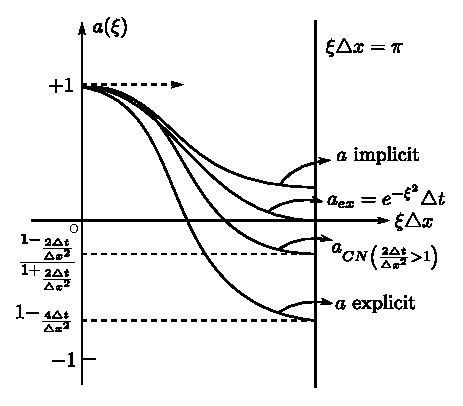
\includegraphics{figures/fig52-7.1.eps}
\caption{}\label{c7:fig7.1}
\end{figure}\pageoriginale

\section{Convergence}\label{chap7:sec7.5}

Given a finite difference scheme we would like  to study the
convergence of the approximate solutions to the true solution as the
mesh is made more and more fine. In other words, one has to study how
the error between the approximate and true solutions behaves. Let $L$
be the approximation of the differential operator, $U$ the approximate
solution and $u$ the exact solution. One then has
\begin{equation*}
\left. 
\begin{aligned}
LU & = 0\\
Lu & = \varepsilon,
\end{aligned}
\right\}\tag{7.15}\label{eq7.15}
\end{equation*}
where\pageoriginale $\varepsilon$ is the error of discretization. The error in the
solution is $e = u- U$ and by virtue of (\ref{eq7.15}) on has 
\begin{equation*}
Le= \varepsilon\tag{7.16}\label{eq7.16}
\end{equation*}

Let us assume that the scheme defined by $L$ is stable, i.e. $||G^n||$
is bounded for all $n$ by a constant, $C(\Delta x, \Delta)$. We are
interested in the case where $C$ is freee of $\Delta x$ and $\Delta t$
as well. This leads us to 

\begin{Definition}\label{chap7:def7.3}
A given scheme is said to be uniformly stable, if the constant $C$
while bounds $||G^n||$ for all $n$, is independent of $\Delta x$ and
$\Delta t$ when $\Delta x \leq \overline{\Delta x}$ and $\Delta t \leq
\overline{\Delta t}$ and $(\Delta x, \Delta  t)$ belonging to the
subspace of $\mathbb{R}^2$ which gives the stability of the scheme. 
\end{Definition}

Let us assume that $L$ gives a uniformly stable scheme in the sense
above and that it is consistent as well. Let us fix any time $t$. Then
divide $[0,t]$ into $n$ equal parts so that $t = n \Delta t$. Let
$e^n$ be the error at time level $n\Delta t$. (Since initial condition
is assumed to be given, one has $e^\circ = 0$). One can then prove
that 
\footnotetext[1]{This is the analogue of remark \ref{chap4:rem4.1} about the fact
  that an energy inequality in the homogieneous case always implies
  the same in the inhomogeneous case. Here energy inequality has to be
replaced by stability. }
$$
||e^n|| \leq C||\varepsilon||. \quad (\footnotemark[1]{})
$$

Let us make $\Delta x$, $\Delta t \to 0$. Then automatically, $n \to
\infty$ for $n \Delta t = t$ fixed. Further $\varepsilon \to 0$, by
consistency. This implies that $||e^n||\to 0$. In other words for each
time $t$, the approximate solutions converge to the exact solution in
whatever norm we have stability. 

This is a sketch of the proof of the fact that (uniform) stability and
consistency imply the convergence of the scheme. This is part of the
Lax's equivalence\pageoriginale theorem which states that stability
and consistency are together equivalent to convergence of a scheme.

For details of this theorem and for more difference schemes, the
reader can refer to Richtmyer and Morton \cite{key32}.


\section{The energy method}\label{chap7:sec7.6}

We now describe another technique for studying stability of difference
schemes. This is know as the {\em energy method}.


\begin{exam}\label{chap7:exam7.6}
Consider the following scheme for the heat equation:
\begin{align*}
&\frac{u^{n+1}_i - u^n_i}{\Delta t} - \frac{1}{\Delta x^2}\\ 
  & \quad \left[ \theta
  (u^{n+1}_{i+1} - 2 u^{n+1}_i + u^{n+1}_{i-1}) + (1-\theta) (u^n_{i+1} - 2
  u^n_i + u^n_{i-1})   \right] =0
\tag{7.17}\label{eq7.17}
\end{align*}
for $0 \leq \theta \leq 1$. (If $\theta = 0$, we get the explicit
scheme; for $\theta =1$ we get the implicit scheme and for $\theta
=\frac{1}{2}$ we have the Crank-Nicolson scheme).

We study stability on the space $\ell^2$, of square summable
sequences. On this space we define the inner product
\begin{equation*}
\langle u,v \rangle  = \Delta x \sum\limits^\infty_{i=-\infty} u_i v_i
\tag{7.18} \label{eq7.18}
\end{equation*}
where $u= (u_i)$, $v= (v_i)$. Then $A: \ell^2 \to \ell^2$ is defined
by 
\begin{equation*}
(Au)_i = - \frac{1}{\Delta x^2} \left[ u_{i+1} - 2 u_i + u_{i-1}
    \right]. \tag{7.19}\label{eq7.19}
\end{equation*}
We may write the equation (\ref{eq7.17}) in vector form as 
\begin{equation*}
\frac{u^{n+1} -u^n}{\Delta t} + A(\theta u^{n+1} + (1-\theta) u^n) =
0. \tag{7.20}\label{eq7.20}
\end{equation*}
Let us denote by $u^*$ the vector $\theta u^{n+1} +
(1-\theta)u^n$. Then we notice that 
\begin{equation*}
2u^* = (u^{n+1} + u^n) + (2\theta -1) (u^{n+1} - u^n) . 
\tag{7.21}\label{eq7.21}
\end{equation*}

One also recalls the familiar identity
\begin{equation*}
\langle a + b, \; a -b\rangle =|a|^2 - |b|^2
\tag{7.22}\label{eq7.22}
\end{equation*}\pageoriginale 
where $|\cdot|$ is the norm induced by the scalar product.

Taking the scalar product of (\ref{eq7.20}) with $2u^*$, one has, using
(\ref{eq7.21}) and (\ref{eq7.22})
$$ 
\frac{|u^{n+1}|^2 - |u^n|^2}{\Delta t} + \left(\frac{2\theta-1}{\Delta t}\right)
|u^{n+1} -u^n|^2 + 2 \langle Au^*, u^*\rangle  = 0. 
$$
Again, using (\ref{eq7.20}) we get 
\begin{equation*}
\frac{|u^{n+1}|^2 - |u^n|^2}{\Delta t} + (2\theta -1) \Delta t
|Au^*|^2 + 2 \langle Au^*, u^*\rangle  = 0.\tag{7.23}\label{eq7.23}
\end{equation*}

A moment's reflection will show that 
\begin{equation*}
\langle Au, u \rangle  = \Delta x \sum\limits_i \left(\frac{u_{i+1} -
  u_i}{\Delta x}\right)^2 \geq 0\tag{7.24}\label{eq7.24}
\end{equation*}

Thus if $\theta \geq \frac{1}{2} $ i.e. $2\theta -1 \geq 0$, we get
from (\ref{eq7.23}) that $|u^{n+1}| \leq |u^n|$ which gives $\ell^2$-stability
of the scheme unconditionally. In particular, this is the case of the
implicit and the Crank-Nicolson schemes. In case $0\leq \theta <
\frac{1}{2}$, the middle term of (\ref{eq7.22}) is negative and thus one
cannot expect unconditional stability.

At this stage one needs the following
\end{exam}

\begin{lem}\label{chap7:lem7.1}
$|Au|^2 \leq \dfrac{4}{\Delta x^2} \langle Au, u\rangle$.
\end{lem}

\begin{proof}
\begin{align*}
|Au|^2 & = \Delta x \sum\limits^\infty_{-\infty} \frac{1}{(\Delta x)^4} (u_{i+1} - 2u_i + u_{i-1})^2\\
& = \Delta x \sum\limits^\infty_{-\infty} \frac{1}{(\Delta x)^2}
\left(\frac{u_{i+1} - u_i}{\Delta x}  - \frac{u_i - u_{i-1}}{\Delta
  x}\right)^2 \\ 
& = \frac{\Delta x}{\Delta x^2} \left[\sum\limits^\infty_{-\infty}
  \left(\frac{u_{i+1} - u_i}{\Delta  x}\right)^2 + \sum\limits^\infty_{-\infty}
  \left(\frac{u_i -u_{i-1}}{\Delta x}\right)^2\right.\\ 
  & \left.\hspace{3cm}+ 2 \sum\limits^\infty_{-\infty}
  \left| \left(\frac{u_{i+1} - u_i}{\Delta x}\right) \left(\frac{u_i
    -u_{i-1}}{\Delta x}\right) \right|  \right].  
\end{align*}
Applying the Cauchy-Schwarz inequality to the last term, one has 
\begin{align*}
|Au|^2  & \leq \frac{4}{\Delta x^2} \sum^\infty_{-\infty} \Delta x
(\frac{u_{i+1} - u_i}{\Delta  x})^2 \\ 
& = \frac{4}{\Delta x^2} \langle Au, u\rangle , \quad \text{ by
  (\ref{eq7.23}) }. 
\end{align*}\pageoriginale  
This proves the lemma.
\end{proof}

Using this lemma we find the condition for stability. In order to have stability, one needs $|u^{n+1}|^2 - |u^n|^2 \leq 0$. In other words, we need
$$
(1- 2\theta) \Delta  t |A u^*|^2 \leq 2 \langle Au^*, u^*\rangle 
$$
But $(1-2\theta) \Delta t |Au^*|^2 \leq (1-2\theta) \dfrac{4\Delta
  t}{\Delta x^2} \langle Au^*, u^*\rangle $, by lemma
\ref{chap7:lem7.1}. Thus the stability condition is 
\begin{equation*}
\frac{4\Delta t (1-2\theta)}{\Delta x^2} \leq 2. \tag{7.25}\label{eq7.25}
\end{equation*}

\begin{remark}\label{chap7:rem7.1}
If $\theta = 0$, we get back, from (\ref{eq7.25}), our original $L^2$-stability condition for the explicit scheme. Thus we see that for all our schemes the $L^2$ and $\ell^2$ stability coditions are the same. However, this is not surprising, for under the correspondence $\{u_i\} \longleftrightarrow $ (piecewise linear function with value $u_i$ at $ i\Delta x$), the $\ell^2$- norm is equivalent to the $L^2$-norm.
\end{remark}

All our preceding work has been under the basic assumption that the
mesh is uniform. The case where the mesh is non-uniform in the
$x$-direction is described in the following exercises. 

\begin{exercise}\label{chap7:exer7.1}
Let $\{x_i\}$ be the nodes of the mesh. Let $x_{i+\frac{1}{2}}$ denote the midpoint of $[x_i, x_{i+1}]$ and $x_{i-\frac{1}{2}}$ that of $[x_{i-1}, x_i]$. Define $A$ by
$$
(Au)_i = \frac{-1}{x_{i-\frac{1}{2}} - x_{i-\frac{1}{2}}} \left[\frac{u_{i+1} - u_i}{x_{i+1} - x_i} - \frac{u_i - u_{i-1}}{x_i - x_{i-1}} \right].
$$
If $\Delta x = \max\limits_i (x_{i+1} - x_i)$, show that 
$$
(Au)_i \sim  \frac{\partial^2 u}{\partial x^2} (x_i) + 0(\Delta x).
$$ \pageoriginale
\end{exercise}

\begin{exercise}\label{chap7:exer7.2}
Define the $\ell^2$-inner product by
$$
\langle u, v\rangle  = \sum\limits_i (x_{i+\frac{1}{2}} - x_{i - \frac{1}{2}}) u_i v_i. 
$$
Then show that
$$
|Au|^2 \leq \frac{4}{\min(x_{i+1} - x_i)^2} \langle Au, u\rangle .
$$
\end{exercise}

\begin{remark}\label{chap7:rem7.2}
In the case of an explicit scheme, viz. $\theta = 0$, we get the
stability condition for the non-uniform mesh as $2 \Delta t \leq
\min(x_{i+1} - x_i)^2$ by virtue of exercise \ref{chap7:exer7.2}. In
general it is found that when looking for stability criteria in a
non-uniform mesh, one can adopt the followig rule of the thumb: 

Find out the condition for the uniform mesh case. Then imposing this
condition locally on each interval of the non-uniform mesh, pick out
the strongest of these as the required stability criterion. 

Thus for the explicit scheme, one has $2\Delta t \leq (x_{i+1} -
x_i)^2$ starting from a  uniform mesh. This leads to the `worst'
condition 
$$
2\Delta t \leq \min\limits_i(x_{i+1} - x_i)^2
$$
which was deduced from the preceding exercises.

A  word of caution! This method is purely heuristic, but generally
works. In some cases one can rigorously prove this heuristic stability
criterion (as in the case of the explicit scheme above) but this is not
always possible. 
\end{remark}

Before closing our discussion of the heat equation, we say a few words about the variable coefficient case and the non-linear case. 

\section{Heat equation with variable coefficients}\label{chap7:sec7.7}

The\pageoriginale  heat equation with variable coefficients reads as
\begin{equation*}
\frac{\partial u}{\partial t} - \frac{\partial }{\partial x} \left(\sigma
(x) \frac{\partial u}{\partial x}\right) = ,\tag{7.26}\label{eq7.26} 
\end{equation*}
where $\sigma (x) \geq \alpha >0$.

This may be also written as
\begin{equation*}
\frac{\partial u}{\partial t} - \frac{\partial u}{\partial x}
\frac{\partial \sigma}{\partial x} - \sigma \frac{\partial^2
  u}{\partial x^2} = 0. \tag{7.27}\label{eq7.27}
\end{equation*}

To set up a discrete scheme, the problem is essentially to approximate
the terms other than $\dfrac{\partial u}{\partial t}$. To do this we
have two approaches, based on (\ref{eq7.26}) and (\ref{eq7.27}). 

The first is the `conservative' scheme based on the form (\ref{eq7.26}). We approximate the terms involving derivatives w.r.t. $x$ by
\begin{equation*}
(A^c u)_i = \frac{-1}{\Delta x^2} \left[\sigma _{i + \frac{1}{2}}  (u_{i+1} - u_i) - \sigma_{i - \frac{1}{2}} (u_i - u_{i-1})\right] 
\tag{7.28}\label{eq7.28}
\end{equation*}
and this is of order $O(\Delta x^2 )$.

The second scheme uses (\ref{eq7.27}) to approximate the derivatives w.r.t. $x$. This is the `non-coservative' scheme given by
\begin{equation*}
(Au^{Nc})_i = \frac{-1}{\Delta x^2} \left[ \frac{(u_{i+1} - u_{i-1})}{2}  \; \frac{(\sigma_{i+1} - \sigma_{i-1})}{2} + \sigma_i (u_{i+1} - 2u_i + u_{i-1})\right] 
\tag{7.29}\label{eq7.29}
\end{equation*}
which is also of second order accuracy.

\begin{remark}\label{chap7:rem7.3}
The equation (\ref{eq7.26}) is essentially a conservation
law. Integrating between $a$ and $b$ w.r.t. $x$, we have  
$$
\int\limits^b_a - \frac{\partial}{\partial x} \left(\sigma
\frac{\partial u}{\partial x}\right) dx = - \sigma (b,t) \frac{\partial u
}{\partial x} (b,t) + \sigma (a,t) \frac{\partial u}{\partial x} (a,t) 
$$
and replacing the term involving $\sigma$ by summation, one has 
\begin{align*}
\Delta x \sum\limits^{i_1}_{i=i_\circ} (A^cu)_i & = -\frac{1}{\Delta
  x} \left[ \sigma_{i+\frac{1}{2}} (u_{i+1} - u_i)\right]_{i=i_1} +
\frac{1}{\Delta x} \left[\sigma_{i-\frac{1}{2}} (u_i -
  u_{i-1}) \right]_{i=i_0} \tag{7.30}\label{eq7.30} 
\end{align*}\pageoriginale
which turns our to be the discreate analogue of (\ref{eq7.30}). If we
use the non-conservative scheme to replace the terms involving
$\sigma$, the summation will  not be `telescopic' to resemble equation
(\ref{eq7.30}). Thus the conservation scheme gives the discrete
analogue of the continuous case and is used in general. 
\end{remark}

One can prove a lemma analogous  to lemma \ref{chap7:lem7.1} and exercise \ref{chap7:exer7.2}. We state it below.

\begin{lem}\label{chap7:lem7.2}
If $A : \ell^2 \to \ell^2$ is defined by (\ref{eq7.28}), then,
\begin{equation*}
|Au|^2 \leq \frac{4}{\Delta x^2} \max\limits_i |\sigma_{i+\frac{1}{2}}| \langle Au, u\rangle  \tag{7.31}\label{eq7.31}
\end{equation*}
\end{lem}

\begin{remark}\label{chap7:rem7.4}
If $\sigma (x) \equiv 1$, we get back lemma \ref{chap7:lem7.1}. We observe that the stability conditions can be made to follow from a heuristic argument similar to that enunciated in remark \ref{chap7:rem7.2}. The stability condition for the explicit scheme will then be
$$
\frac{2\Delta t}{\Delta x^2} \max\limits_i |\sigma_{i+\frac{1}{2}}| \leq 1
$$
which, in this case, can be proved using lemma \ref{chap7:lem7.2}.
\end{remark}

\section{A non-linear example}\label{chap7:sec7.8}

The non-linear heat equation is of the form
\begin{equation*}
\frac{\partial u}{\partial t} - \frac{\partial}{\partial x} \left(\sigma
(u) \frac{\partial u}{\partial x}\right) = 0 .\tag{7.32}\label{eq7.32} 
\end{equation*}

If $\sigma \geq 0$, $\sigma \in C^1$ and $0 < \alpha \leq \sigma (u)
\leq \beta$, then one can imitate the analysis of Section
\ref{chap7:sec7.7}. of the linear case. However, if $\alpha =0$, then
such techniques do not extend to the non-linear
equation. Nevertheless, particular forms of $\sigma (u)$ have
been\pageoriginale studied. 

We consider the case where $\sigma (u) = mu^{m-1} $, $u \geq 0$,
$m>1$. The condition $u\geq 0$ is the one that is encountered in
physics since $u$ is the temperature. Then the equation can be written
as  
\begin{equation*}
\frac{\partial u}{\partial t} - \frac{\partial^2 u^m}{\partial x^2} = 0,
\tag{7.33}\label{eq7.33}
\end{equation*}
with the initial condition, say, $u(x,0) =0$, and boundary condition
given by prescribing either $u(0,t)$ or $\dfrac{\partial u^m}{\partial
  n} (0,t) = - \frac{\partial u^m}{\partial x} (0,t)$ (the normal
derivative on $x=0$), both non-negative so as to ensure, by the
maximum principle, that the solution $u$ will be $\geq 0$
everywhere. For a given $t$, the solution will take the form as shown
in Fig. \ref{c7:fig7.2}.  
\begin{figure}[H]
\centering
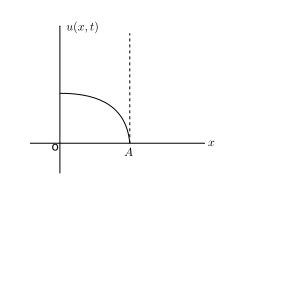
\includegraphics{figures/fig52-7.2.eps}
\caption{}\label{c7:fig7.2}
\end{figure}

In the case $m \geq 2$, the derivative of $u$ at $A$ is
infinite. However there is a result due to Aronson \cite{key3} which
states that $u^{m-1}$ has bounded derivatives. Hence to set up an
approximate scheme we rewrite (\ref{eq7.33}) as  
\begin{equation*}
\frac{\partial u}{\partial t} - \frac{\partial}{\partial x}
\left(\frac{mu}{m-1} \frac{\partial u^{m-1}}{\partial x}\right) =
0.\tag{7.34}\label{eq7.34} 
\end{equation*}

Now we\pageoriginale approximate the term involving derivatives w.r.t. $x$ by
\begin{align*}
(Au)_i & = \frac{-m}{\Delta x(m-1)} \left[ \left(\frac{u^{m-1}_{i+1} +
      u^{m-1}_i}{2}\right)^{\frac{1}{m-1}} \left(\frac{u^{m-1}_{i+1} -
      u^{m-1}_{i}}{\Delta x}\right)+ \right.\\  
& \hspace{2.5cm} + \left. \left(\frac{u^{m-1}_i +
      u^{m-1}_{i-1}}{2}\right)^{\frac{1}{m-1}} 
    \left(\frac{u^{m-1}_i - u^{m-1}_{i-1}}{\Delta x}\right)
    \right]. \tag{7.35} \label{eq7.35} 
\end{align*}

Notice that we use again the ``almost linearity'' of $u^{m-1}$ to
define a value $u_{i+\frac{1}{2}}$ interpolated between $u_i$ and
$u_{i+1}$. From this we can generate various implicit and explicit
schemes. For example, the implicit scheme will read as 
\begin{equation*}
\frac{u^{n-1}_i - u^n_i}{\Delta t} + (Au^{n+1})_i = 0
\tag{7.36}\label{eq7.36}
\end{equation*}
which is, w.r.t. the unknown at time $(n+1)\Delta t$, of the form 
\begin{equation*}
F_i (u^{n+1}_{i+1},u^{n+1}_i, u^{n+1}_{i-1}) = 0.
\tag{7.37}\label{eq7.37}
\end{equation*}

So we get a non-linear (``tridiagonal'') system to solve and this
could be done by Newton's method of linearising locally, so that at
each iteration one has to solve a linear tridiagonal system, which is
easy. 

If one wants to use the explicit scheme (given by $\frac{u^{n+1}_i -
  u^n_i}{\Delta t} + (Au^n)_i = 0$), in order to avoid solving linear
systems one would get the heuristic stability condition 
\begin{equation*}
2m \; \max |u|^{m-1} \frac{\Delta t}{\Delta x^2} \leq 1\tag{7.38}\label{eq7.38}
\end{equation*}
which can be very drastic.

For non-linear examples see also Graveleau and Jamet \cite{key14}.
